\chapter{Prototipo 1}
\section{Modelo de datos}
\paragraph{Dentro del modelo de la aplicación final se toma en cuenta el modelo general mínimo necesario para trabajar la información añadiendo información relevante sobre el caso de estudio que recae en platillos como articulos a recomendar. Considerando al final las siguientes entidades.}

\begin{itemize}
  \item Platillos
  \item Usuarios
  \item Restaurantes
  \item Categorias 
\end{itemize}

\paragraph{Para la información de los restaurantes, el modelo  permitirá almacenar una fuente de información externa en caso de ser utilizada, para obtener datos adicionales a los que se poseen en la base de datos de acuerdo a registros como pueden ser los contenidos por Foursquare en su API para la búsqueda de restaurantes.}

\paragraph{Las relaciones posibles entre los elementos Usuario, Restaurante, Platillo y sus posibles Categorias son visualizados en el siguiente diagrama.}

\newpage
    \begin{landscape}
      \begin{figure}[h!]
      \centering
      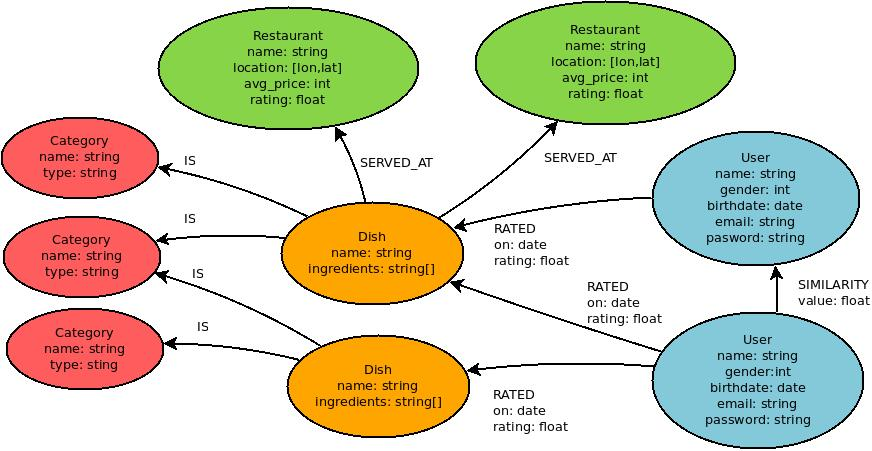
\includegraphics[width=22.5cm,height=12cm]{./images/Modelo_datos.jpg}
      \caption{Modelo propuesto para el caso de estudio}
    \end{figure}
    \end{landscape}
  \newpage

\newpage
\subsubsection{Modelo de datos}
  \lstinputlisting[language=Javascript]{../Resources/Model.js} 

\newpage
\subsubsection{Categorias propuestas}
  \lstinputlisting[language=Javascript]{../Resources/Categories.js} 